\section{\methodfull}

\begin{figure*}[ht]
    \centering
    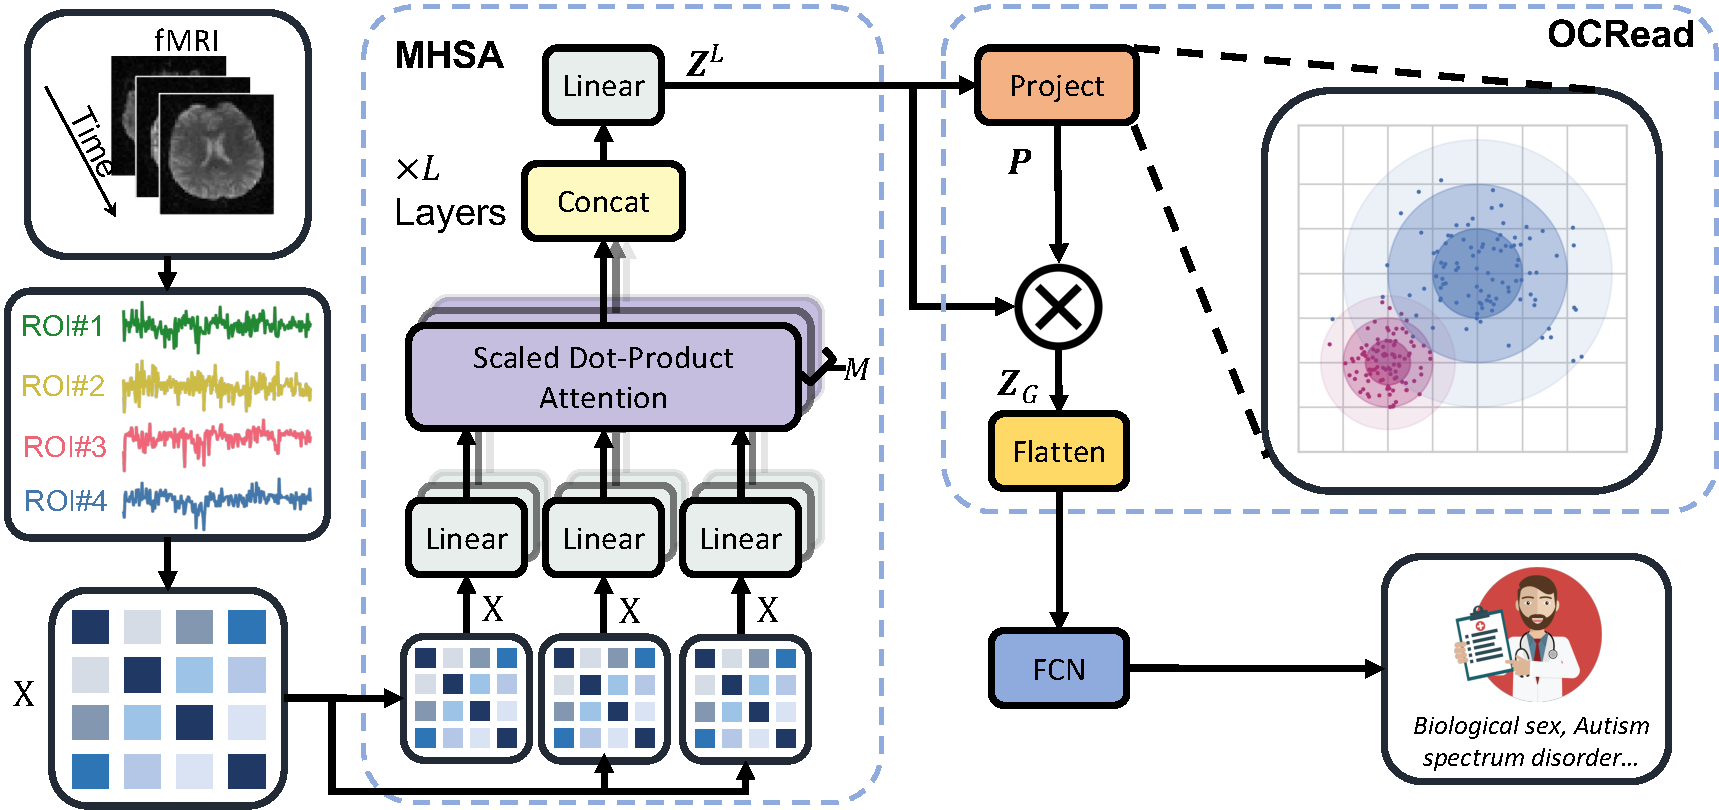
\includegraphics[width=0.8\linewidth]{figures/process.pdf}
    \caption{The overall framework of our proposed \methodfull.}
    \label{fig:model}
\end{figure*}

\subsection{Problem Definition}
In brain network analysis, given a brain network $\bm X\in \mathbb{R}^{V \times V}$, where $V$ is the number of nodes (ROIs), the model aims to make a prediction indicating biological sex, presence of a disease or other properties of the brain subject. The overall framework of our proposed \methodfull is shown in Figure \ref{fig:model}, which is mainly composed of two components, an $L$-layer attention module $\operatorname{MHSA}$ and a graph pooling operator \poolingshort.
Specifically, in the first component of $\operatorname{MHSA}$, the model learns attention-enhanced node features $\bm Z^L$ through a non-linear mapping $\bm X \rightarrow \bm Z^L \in \mathbb{R}^{V \times V}$. Then the second component of \poolingshort compresses the enhanced node embeddings $\bm Z^L$ to graph-level embeddings $\bm Z_G \in \mathbb{R}^{K \times V}$, where $K$ is a hyperparameter representing the number of clusters. $\bm Z_G$ is then flattened and passed to a multi-layer perceptron for graph-level predictions. The whole training process is supervised with the cross-entropy loss.

\subsection{Multi-Head Self-Attention Module (MHSA)}
To develop a powerful Transformer-based model suitable for brain networks, two fundamental designs, the positional embedding and attention mechanism, need to be reconsidered to fit the natural properties of brain network data. In existing graph transformer models, the positional information is usually encoded via eigendecomposition, while the attention mechanism often combines node positions with existing edges to calculate the attention scores. However, for the dense (often fully connected) graphs of brain networks, eigendecomposition is rather costly, and the existence of edges is hardly informative.

ROI node features on brain networks naturally contain sufficient positional information, making the positional embeddings based on eigendecomposition redundant. Previous work on brain network analysis has shown that the connection profile $\bm X_{i\cdot}$ for node $i$, defined as the corresponding row for each node in the edge weight matrix $\bm X$, always achieves superior performance over others such as node identities, degrees or eigenvector-based embeddings \citep{li2020braingnn, kan2022fbnetgen, braingb}. With this node feature initialization, the self-connection weight $\bm x_{ii}$ on the diagonal is always equal to one, which encodes sufficient information to determine the position of each node in a fully connected graph based on the given brain atlas.
To verify this insight, we also empirically compare the performance of the original connection profile with two variants concatenated with additional positional information, \textit{i.e.}, connection profile w/ identity feature and connection profile w/ eigen feature. The results indeed show no benefit brought by the additional computations (c.f.~Appendix \ref{app:node_feature}).
As for the attention mechanism, previous work \citep{braingb} has empirically demonstrated that integrating edge weights into the attention score calculation can significantly degrade the effectiveness of attention on complete graphs, while the generation of edge-wise embedding can be unaffordable given a large number of edges in brain networks. On the other hand, the existence of edges provides no useful information for the computation of attention scores as well because all edges simply exist in complete graphs.

Based on the observations above, we design the basic \methodfull by (1) adopting the connection profile as initial node features and eliminating any extra positional embeddings and (2) adopting the vanilla pair-wise attention mechanism without using edge weights or relative position information to learn a singular attention score for each edge in the complete graph.

Formally, we leverage a $L$-layer non-linear mapping module, namely Multi-Head Self-Attention ($\operatorname{MHSA}$), to generate more expressive node features $\bm Z^L = \operatorname{MHSA}(\bm X) \in \mathbb{R}^{V \times V}$. For each layer $l$, the output $\bm Z^{l}$ is obtained by
\begin{equation}
% \begin{array}{c}
\bm Z^{l} = (\Vert_{m=1}^{M}{\bm h^{l,m}})\bm W^l_{\mathcal{O}},
\text {} \bm h^{l,m} =\operatorname{Softmax}\left(\frac{\bm W_{\mathcal{Q}}^{l, m} \bm Z^{l-1} (\bm W_{\mathcal{K}}^{l, m} \bm Z^{l-1})^{\top}}{\sqrt{d_{\mathcal{K}}^{l, m}}}\right) \bm W_{\mathcal{V}}^{l, m} \bm Z^{l-1},
% \end{array}
\end{equation}
where $\bm Z^0 = \bm X$, $\Vert$ is the concatenation operator, $M$ is the number of heads, $l$ is the layer index, $\bm W^l_{\mathcal{O}}, \bm W_{\mathcal{Q}}^{l, m}, \bm W_{\mathcal{K}}^{l, m}$, $\bm W_{\mathcal{V}}^{l, m}$ are learnable model parameters, and $d_{\mathcal{K}}^{l, m}$ is the first dimension of $\bm W_{\mathcal{K}}^{l, m}$.

\subsection{\pooling (\poolingshort)}

The readout function is an essential component to learn the graph-level representations for brain network analysis (\textit{e.g.}, classification), which maps a set of learned node-level embeddings to a graph-level embedding. $\operatorname{Mean}(\cdot), \operatorname{Sum}(\cdot)$ and $\operatorname{Max}(\cdot)$ are the most commonly used readout functions for GNNs. Xu et al. \citep{xu_sum} show that GNNs equipped with $\operatorname{Sum}(\cdot)$ readout have the same discriminative power as the Weisfeiler-Lehman Test. Zhang et al. \citep{zhang2018end} propose a sort pooling to generate the graph-level representation by sorting the final node representations. Ju et al. \citep{liangzhao} present a layer-wise readout by extending the node information aggregated from the last layer of GNNs to all layers. However, none of the existing readout functions leverages the properties of brain networks that nodes in the same functional modules tend to have similar behaviors and clustered representations, as shown in Figure \ref{fig:motivation}(a). To address this deficiency, we design a novel readout function to take advantage of the modular-level similarities between ROIs in brain networks, where nodes are assigned softly to well-chosen clusters with an unsupervised process. 

Formally, given $K$ cluster centers, each center has $V$ dimensions, $\bm E\in \mathbb{R}^{K \times V }$, a Softmax projection operator is used as the function to calculate the probability $\bm P_{ik}$ of assigning node $i$ to cluster $k$, 
\begin{equation}
\label{equ:project}
\bm P_{ik} =\frac{e^{\langle \bm Z_{i\cdot}^L, \bm E_{k\cdot}\rangle} }{\sum_{k^{\prime}}^K e^{\langle \bm Z_{i\cdot}^L, \bm E_{k^{\prime}\cdot}\rangle}}, 
\end{equation}
where $\langle \cdot, \cdot\rangle$ denotes the inner product and $\bm Z^L$ is the learned set of node embeddings from the last layer of $\operatorname{MHSA}$ module. With this computed soft assignment $\bm P\in \mathbb{R}^{V \times K }$, the original learned node representation $\bm Z^L$ can be aggregated under the guidance of the soft cluster information, where the graph-level embedding $\bm Z_G$ is obtained by $\bm Z_G=\bm P^\top \bm Z^L$.

However, jointly learning node embeddings and clusters without ground-truth cluster labels is difficult. To obtain representative soft assignment $\bm P$, the initialization of $K$ cluster centers $\bm E$ is critical and should be designed delicately. To this end, we leverage the observation illustrated in Figure \ref{fig:motivation}(b), where orthonormal embeddings can improve the clustering of nodes in brain networks \textit{w.r.t.}~the functional modules underlying brain regions.

\textbf{Orthonormal Initialization}. To initialize a group of orthonormal bases as cluster centers, we first adopt the Xavier uniform initialization~\citep{glorot2010understanding} to initialize $K$ random centers and each center contains $V$ dimensions $\bm C\in \mathbb{R}^{K \times V }$. Then, we apply the Gram-Schmidt process to obtain the orthonormal bases $\bm E$, where
\begin{equation}
\label{equ:otho}
\bm u_{k}=\bm C_{k\cdot}-\sum_{j=1}^{k-1} \frac{\langle \bm u_{j}, \bm C_{k\cdot}\rangle }{\langle \bm u_{j},\bm u_{j}\rangle}\bm u_{j}, \quad \bm E_{k\cdot}=\frac{\bm u_{k}}{\left\|\bm u_{k}\right\|}.
\end{equation}

In the next section, we theoretically prove the advantage of this orthonormal initialization.


\subsubsection{Theoretical Justifications} \label{sec:theoretical}

In \poolingshort, proper cluster centers can generate higher-quality soft assignments and enlarge the difference between $\bm P$ from different classes. \citep{Saxe2014ExactST, haitao} showed the advantages of orthogonal initialization in DNN model parameters. However, none of them proves whether it is an ideal strategy to obtain the cluster centers. We propose two methods from the perspective of statistics as follows. 

Firstly, to discern features of different nodes, we would expect a larger discrepancy among their similarity probabilities indicated from the readout. One way to measure the discrepancy is using the \emph{variance} of $\bm P$ for each feature. Let $\bar{\bm P} \equiv 1/K$ denote the mean of any discrete probabilities with $K$ values. Variance of $\bm P$ measures the difference between $\bm P$ and $\bar{\bm P}$. We average over the feature vector space: if the result is small, then there is a large tendency that different $\bm P$ approaches $\bar{\bm P}$ and hence cannot be discerned easily. Specifically, the following theorem holds for our function Eq.~\eqref{equ:project}:
\begin{theorem} \label{Thm3.1}
	For arbitrary $r > 0$, let $B_r = \{\mathcal{\bm Z} \in \mathbb{R}^V; \Vert \mathcal{\bm Z} \Vert \leq r\}$ denote the round ball centered at origin of radius $r$ with $\mathcal{\bm Z}$ being fracture vectors. Let $V_r$ be the volume of $B_r$. The variance of Softmax projection averaged over $B_r$
	\begin{align}
		\frac{1}{V_r} \int_{B_r} \sum_k^K \Big( \frac{e^{\langle \mathcal{\bm Z}, \bm E_{k\cdot}\rangle} }{\sum_{k^{\prime}}^K e^{\langle \mathcal{\bm Z}, \bm E_{k^{\prime}\cdot}\rangle}} - \frac{1}{K} \Big)^2 d \mathcal{\bm Z},
	\end{align}
    attains maximum when $\bm E$ is orthonormal.
\end{theorem}
Despite the concise form, it is unclear whether the above integral has an elementary antiderivative. Even though, we can circumvent this problem and a rigorous proof is given in Appendix \ref{app:prove}.

The second statistical method shows that for general readout functions without a known analytical form, initializing with orthonormal cluster centers has a larger probability of gaining better performance. To set up the proper statistical scenario, we assume that the unknown readout is obtained by a regression of some samples $(\hat{\bm Z}^{(s)}, \hat{\bm E}^{(t)}, \hat{\bm P}^{(st)})$. This formally converts the exact functional relationship between $\bm Z_{i\cdot}, \bm E_{k\cdot}$ and $\bm P_{ik}$ to a \emph{statistical relationship}:
\begin{align}
	\bm P_T(\bm Z_{i\cdot}, \bm E_{k\cdot}) = \bm P(\bm Z_{i\cdot}, \bm E_{k\cdot}) + \epsilon_i, \quad \epsilon_i \sim N(0,\sigma^2), \quad  E(\epsilon_i) = 0,  \quad  D(\epsilon_i) = \sigma^2, 
\end{align}
with $\bm P_T$ being the probability \emph{truly} reflecting similarities between nodes and clusters and $\epsilon_i$ denoting the stochastic error. It is almost impossible to find $\bm P_T$, but by computing the so-called \emph{variation inflation factor} \cite{Kutner1985}, we show that regression in orthonormal case has a higher accuracy than that in non-orthonormal case. Combining with a hypothesis testing, we obtain the following 
\begin{theorem} \label{Thm3.2}
	The significance level $\alpha_{E_{k\cdot}}$ which reveals the probability of rejecting a well-estimated pooling is lower when sampling from orthonormal centers than that from non-orthonormal centers.
\end{theorem}
More details can be seen in Appendix \ref{app:prove}.

\subsection{Generalizing \poolingshort to Other Graph Tasks and Domains}

In this work, we tested the proposed \poolingshort on functional connectivity (FC) based brain networks. Other popular modalities of brain networks include structural connectivities (SC), which describe the anatomical organization of the brain by measuring the fiber tracts between brain regions \citep{10.3389/fnhum.2021.721206}. In SC-based brain networks, ROIs that are positionally close to each other on the structural connectivity networks tend to share similar connection profiles. This means the idea of \poolingshort is also naturally applicable to SC networks, where the orthonormal clustering is based on the physical distances instead of the functional modules on FC. 

At a higher level, the idea of our proposed \poolingshort is not confined to graph-level prediction tasks on brain networks but can also be generalized to other graph learning tasks and domains. Precisely, there is a growing tendency in node/edge level prediction tasks to enhance the node/edge representation learning by utilizing the subgraph embeddings around each target node/edge \citep{NEURIPS2021_8462a7c2, linkprediction}. In this process, substructure learning needs to be performed on the subgraphs, where our proposed \poolingshort can be adapted for compressing a set of node embeddings to subgraph embeddings. 
Besides, \poolingshort is also potentially useful for other types of graphs in the biomedical domains. For example, for protein-protein interaction networks, proteins can be implicitly grouped by families that share common evolutionary origins \citep{10.1093/nar/gkaa913}, whereas for gene expression networks, genes can be grouped based on the latent pathway information \citep{kanehisa2000kegg}. Both of them are potential directions for the future application of \poolingshort, among many others driven by biological or other types of prior knowledge regarding underlying node/edge groups.
